\section{eo\-Ranking$<$ EOT $>$ Class Template Reference}
\label{classeo_ranking}\index{eoRanking@{eoRanking}}
An instance of eo\-Perf\-From\-Worth COmputes the ranked fitness: fitnesses range in [m,M] with m=2-pressure/pop\-Size and M=pressure/pop\-Size.  


{\tt \#include $<$eo\-Ranking.h$>$}

Inheritance diagram for eo\-Ranking$<$ EOT $>$::\begin{figure}[H]
\begin{center}
\leavevmode
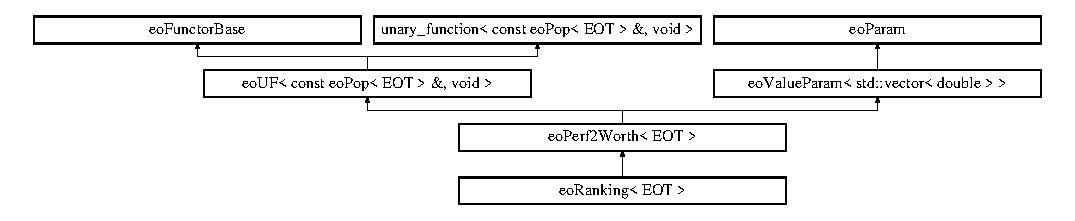
\includegraphics[height=2.52252cm]{classeo_ranking}
\end{center}
\end{figure}
\subsection*{Public Member Functions}
\begin{CompactItemize}
\item 
{\bf eo\-Ranking} (double \_\-p=2.0, double \_\-e=1.0)\label{classeo_ranking_a0}

\item 
int {\bf lookfor} (const {\bf EOT} $\ast$\_\-eo, const {\bf eo\-Pop}$<$ {\bf EOT} $>$ \&\_\-pop)\label{classeo_ranking_a1}

\item 
virtual void {\bf operator()} (const {\bf eo\-Pop}$<$ {\bf EOT} $>$ \&\_\-pop)\label{classeo_ranking_a2}

\begin{CompactList}\small\item\em The pure virtual function that needs to be implemented by the subclass. \item\end{CompactList}\end{CompactItemize}
\subsection*{Private Attributes}
\begin{CompactItemize}
\item 
double {\bf pressure}\label{classeo_ranking_r0}

\item 
double {\bf exponent}\label{classeo_ranking_r1}

\end{CompactItemize}


\subsection{Detailed Description}
\subsubsection*{template$<$class EOT$>$ class eo\-Ranking$<$ EOT $>$}

An instance of eo\-Perf\-From\-Worth COmputes the ranked fitness: fitnesses range in [m,M] with m=2-pressure/pop\-Size and M=pressure/pop\-Size. 

in between, the progression depstd::ends on exponent (linear if 1). 



Definition at line 38 of file eo\-Ranking.h.

The documentation for this class was generated from the following file:\begin{CompactItemize}
\item 
eo\-Ranking.h\end{CompactItemize}
